\documentclass[]{article}
\usepackage{lmodern}
\usepackage{amssymb,amsmath}
\usepackage{ifxetex,ifluatex}
\usepackage{fixltx2e} % provides \textsubscript
\ifnum 0\ifxetex 1\fi\ifluatex 1\fi=0 % if pdftex
  \usepackage[T1]{fontenc}
  \usepackage[utf8]{inputenc}
\else % if luatex or xelatex
  \ifxetex
    \usepackage{mathspec}
  \else
    \usepackage{fontspec}
  \fi
  \defaultfontfeatures{Ligatures=TeX,Scale=MatchLowercase}
\fi
% use upquote if available, for straight quotes in verbatim environments
\IfFileExists{upquote.sty}{\usepackage{upquote}}{}
% use microtype if available
\IfFileExists{microtype.sty}{%
\usepackage{microtype}
\UseMicrotypeSet[protrusion]{basicmath} % disable protrusion for tt fonts
}{}
\usepackage[margin=1in]{geometry}
\usepackage{hyperref}
\hypersetup{unicode=true,
            pdftitle={Explicacion aplicacion},
            pdfauthor={Willmer},
            pdfborder={0 0 0},
            breaklinks=true}
\urlstyle{same}  % don't use monospace font for urls
\usepackage{color}
\usepackage{fancyvrb}
\newcommand{\VerbBar}{|}
\newcommand{\VERB}{\Verb[commandchars=\\\{\}]}
\DefineVerbatimEnvironment{Highlighting}{Verbatim}{commandchars=\\\{\}}
% Add ',fontsize=\small' for more characters per line
\usepackage{framed}
\definecolor{shadecolor}{RGB}{248,248,248}
\newenvironment{Shaded}{\begin{snugshade}}{\end{snugshade}}
\newcommand{\AlertTok}[1]{\textcolor[rgb]{0.94,0.16,0.16}{#1}}
\newcommand{\AnnotationTok}[1]{\textcolor[rgb]{0.56,0.35,0.01}{\textbf{\textit{#1}}}}
\newcommand{\AttributeTok}[1]{\textcolor[rgb]{0.77,0.63,0.00}{#1}}
\newcommand{\BaseNTok}[1]{\textcolor[rgb]{0.00,0.00,0.81}{#1}}
\newcommand{\BuiltInTok}[1]{#1}
\newcommand{\CharTok}[1]{\textcolor[rgb]{0.31,0.60,0.02}{#1}}
\newcommand{\CommentTok}[1]{\textcolor[rgb]{0.56,0.35,0.01}{\textit{#1}}}
\newcommand{\CommentVarTok}[1]{\textcolor[rgb]{0.56,0.35,0.01}{\textbf{\textit{#1}}}}
\newcommand{\ConstantTok}[1]{\textcolor[rgb]{0.00,0.00,0.00}{#1}}
\newcommand{\ControlFlowTok}[1]{\textcolor[rgb]{0.13,0.29,0.53}{\textbf{#1}}}
\newcommand{\DataTypeTok}[1]{\textcolor[rgb]{0.13,0.29,0.53}{#1}}
\newcommand{\DecValTok}[1]{\textcolor[rgb]{0.00,0.00,0.81}{#1}}
\newcommand{\DocumentationTok}[1]{\textcolor[rgb]{0.56,0.35,0.01}{\textbf{\textit{#1}}}}
\newcommand{\ErrorTok}[1]{\textcolor[rgb]{0.64,0.00,0.00}{\textbf{#1}}}
\newcommand{\ExtensionTok}[1]{#1}
\newcommand{\FloatTok}[1]{\textcolor[rgb]{0.00,0.00,0.81}{#1}}
\newcommand{\FunctionTok}[1]{\textcolor[rgb]{0.00,0.00,0.00}{#1}}
\newcommand{\ImportTok}[1]{#1}
\newcommand{\InformationTok}[1]{\textcolor[rgb]{0.56,0.35,0.01}{\textbf{\textit{#1}}}}
\newcommand{\KeywordTok}[1]{\textcolor[rgb]{0.13,0.29,0.53}{\textbf{#1}}}
\newcommand{\NormalTok}[1]{#1}
\newcommand{\OperatorTok}[1]{\textcolor[rgb]{0.81,0.36,0.00}{\textbf{#1}}}
\newcommand{\OtherTok}[1]{\textcolor[rgb]{0.56,0.35,0.01}{#1}}
\newcommand{\PreprocessorTok}[1]{\textcolor[rgb]{0.56,0.35,0.01}{\textit{#1}}}
\newcommand{\RegionMarkerTok}[1]{#1}
\newcommand{\SpecialCharTok}[1]{\textcolor[rgb]{0.00,0.00,0.00}{#1}}
\newcommand{\SpecialStringTok}[1]{\textcolor[rgb]{0.31,0.60,0.02}{#1}}
\newcommand{\StringTok}[1]{\textcolor[rgb]{0.31,0.60,0.02}{#1}}
\newcommand{\VariableTok}[1]{\textcolor[rgb]{0.00,0.00,0.00}{#1}}
\newcommand{\VerbatimStringTok}[1]{\textcolor[rgb]{0.31,0.60,0.02}{#1}}
\newcommand{\WarningTok}[1]{\textcolor[rgb]{0.56,0.35,0.01}{\textbf{\textit{#1}}}}
\usepackage{graphicx,grffile}
\makeatletter
\def\maxwidth{\ifdim\Gin@nat@width>\linewidth\linewidth\else\Gin@nat@width\fi}
\def\maxheight{\ifdim\Gin@nat@height>\textheight\textheight\else\Gin@nat@height\fi}
\makeatother
% Scale images if necessary, so that they will not overflow the page
% margins by default, and it is still possible to overwrite the defaults
% using explicit options in \includegraphics[width, height, ...]{}
\setkeys{Gin}{width=\maxwidth,height=\maxheight,keepaspectratio}
\IfFileExists{parskip.sty}{%
\usepackage{parskip}
}{% else
\setlength{\parindent}{0pt}
\setlength{\parskip}{6pt plus 2pt minus 1pt}
}
\setlength{\emergencystretch}{3em}  % prevent overfull lines
\providecommand{\tightlist}{%
  \setlength{\itemsep}{0pt}\setlength{\parskip}{0pt}}
\setcounter{secnumdepth}{0}
% Redefines (sub)paragraphs to behave more like sections
\ifx\paragraph\undefined\else
\let\oldparagraph\paragraph
\renewcommand{\paragraph}[1]{\oldparagraph{#1}\mbox{}}
\fi
\ifx\subparagraph\undefined\else
\let\oldsubparagraph\subparagraph
\renewcommand{\subparagraph}[1]{\oldsubparagraph{#1}\mbox{}}
\fi

%%% Use protect on footnotes to avoid problems with footnotes in titles
\let\rmarkdownfootnote\footnote%
\def\footnote{\protect\rmarkdownfootnote}

%%% Change title format to be more compact
\usepackage{titling}

% Create subtitle command for use in maketitle
\providecommand{\subtitle}[1]{
  \posttitle{
    \begin{center}\large#1\end{center}
    }
}

\setlength{\droptitle}{-2em}

  \title{Explicacion aplicacion}
    \pretitle{\vspace{\droptitle}\centering\huge}
  \posttitle{\par}
    \author{Willmer}
    \preauthor{\centering\large\emph}
  \postauthor{\par}
      \predate{\centering\large\emph}
  \postdate{\par}
    \date{25/10/2020}


\begin{document}
\maketitle

\hypertarget{tablero-prueba-analista-de-inversion}{%
\subsubsection{TABLERO PRUEBA ANALISTA DE
INVERSION}\label{tablero-prueba-analista-de-inversion}}

El Siguiente documento pretende ilustrar una presentación básica de cómo
está construido el tablero en shiny.

El tablero está dividido en tres partes

\begin{enumerate}
\def\labelenumi{\arabic{enumi}.}
\item
  El procesamiento de los datos: Que abarca las descargas automáticas de
  los datos y la respectiva depuración y preparacion de los datos
\item
  El diseño de la interfaz de usuario
\item
  Las acciones del servidor de R haciendo reactivo cada uno de sus
  elementos
\end{enumerate}

\hypertarget{procesamiento-de-los-datos}{%
\subsection{Procesamiento de los
datos}\label{procesamiento-de-los-datos}}

La descarga de los datos se realiza directamente desde la web la TRM
mediante servicios expuestos que tiene el gobierno nacional a través
socrata y el portal www.datos.gov.co. El precio del petróleo igualmente
mediante los servicios expuesto en la página kapsarc.org Y los datos de
las acciones se descargan automáticamente mediante la librería
BatchGetSymbols

\begin{Shaded}
\begin{Highlighting}[]
\CommentTok{# Ejemplo de descarga y procesamiento}
\KeywordTok{library}\NormalTok{(RSocrata)}
\end{Highlighting}
\end{Shaded}

\begin{verbatim}
## Warning: package 'RSocrata' was built under R version 3.6.3
\end{verbatim}

\begin{Shaded}
\begin{Highlighting}[]
\NormalTok{TRM2 <-}\StringTok{ }\KeywordTok{read.socrata}\NormalTok{(}\StringTok{"https://www.datos.gov.co/resource/ceyp-9c7c.csv"}\NormalTok{)}
\NormalTok{oil2 =}\StringTok{ }\KeywordTok{read.csv}\NormalTok{(}\StringTok{"https://datasource.kapsarc.org/explore/dataset/opec-crude-oil-price/download/?format=csv&timezone=America/Bogota&lang=en&use_labels_for_header=true&csv_separator=%3B"}\NormalTok{ ,}
               \DataTypeTok{sep =} \StringTok{";"}\NormalTok{)}
\NormalTok{oil <-}\StringTok{ }\NormalTok{oil2}
\NormalTok{TRM <-}\StringTok{ }\NormalTok{TRM2}
\NormalTok{oil}\OperatorTok{$}\NormalTok{Date <-}\StringTok{ }\KeywordTok{as.POSIXct}\NormalTok{(oil}\OperatorTok{$}\NormalTok{Date, }\DataTypeTok{format =} \StringTok{"%Y-%m-%d"}\NormalTok{)}
\NormalTok{TRM <-}\StringTok{  }\NormalTok{TRM[}\KeywordTok{order}\NormalTok{(}\KeywordTok{as.Date}\NormalTok{(TRM}\OperatorTok{$}\NormalTok{vigenciadesde, }\DataTypeTok{format=}\StringTok{"%Y-%m-%d"}\NormalTok{)),]}
\NormalTok{oil <-}\StringTok{  }\NormalTok{oil[}\KeywordTok{order}\NormalTok{(}\KeywordTok{as.Date}\NormalTok{(oil}\OperatorTok{$}\NormalTok{Date, }\DataTypeTok{format =} \StringTok{"%Y-%m-%d"}\NormalTok{)),]}
\NormalTok{oil <-}\StringTok{  }\NormalTok{oil[oil}\OperatorTok{$}\NormalTok{Date }\OperatorTok{>=}\StringTok{ '2008-01-01'}\NormalTok{,]}
\NormalTok{TRM <-}\StringTok{  }\NormalTok{TRM[TRM}\OperatorTok{$}\NormalTok{vigenciadesde }\OperatorTok{>=}\StringTok{ '2008-01-01'}\NormalTok{,]}
\NormalTok{copvsoil <-}\StringTok{ }\KeywordTok{merge}\NormalTok{(}\DataTypeTok{x =}\NormalTok{ TRM , }\DataTypeTok{y =}\NormalTok{ oil , }\DataTypeTok{by.x =} \StringTok{"vigenciadesde"}\NormalTok{ , }\DataTypeTok{by.y =} \StringTok{"Date"}\NormalTok{, }\DataTypeTok{all =} \OtherTok{FALSE}\NormalTok{ )}
\NormalTok{copvsoil}\OperatorTok{$}\NormalTok{año <-}\StringTok{ }\KeywordTok{format}\NormalTok{(copvsoil}\OperatorTok{$}\NormalTok{vigenciadesde , }\DataTypeTok{format =} \StringTok{"%Y"}\NormalTok{)}
\NormalTok{copvsoil}\OperatorTok{$}\NormalTok{mes <-}\StringTok{ }\KeywordTok{format}\NormalTok{(copvsoil}\OperatorTok{$}\NormalTok{vigenciadesde , }\DataTypeTok{format =} \StringTok{"%Y-%m"}\NormalTok{)}
\NormalTok{copvsoil}\OperatorTok{$}\NormalTok{mesnum <-}\StringTok{ }\KeywordTok{format}\NormalTok{(copvsoil}\OperatorTok{$}\NormalTok{vigenciadesde , }\DataTypeTok{format =} \StringTok{"%m"}\NormalTok{)}

\KeywordTok{head}\NormalTok{(copvsoil)}
\end{Highlighting}
\end{Shaded}

\begin{verbatim}
##   vigenciadesde   valor vigenciahasta Crude.Oil.Price  año     mes mesnum
## 1    2008-01-03 2012.82    2008-01-03           93.67 2008 2008-01     01
## 2    2008-01-04 2013.27    2008-01-04           93.38 2008 2008-01     01
## 3    2008-01-09 2000.91    2008-01-09           91.98 2008 2008-01     01
## 4    2008-01-10 2004.70    2008-01-10           89.71 2008 2008-01     01
## 5    2008-01-11 2003.74    2008-01-11           88.36 2008 2008-01     01
## 6    2008-01-15 1949.43    2008-01-15           88.33 2008 2008-01     01
\end{verbatim}

Luego de tener los datos financieros y hacer las transformaciones
necesarias que pueden encontrar mas detallado en el codigo de la
aplicacion nos disponer a plantear la interfaz grafica.

\hypertarget{el-diseno-de-la-interfaz-de-usuario}{%
\subsection{2. El diseño de la interfaz de
usuario}\label{el-diseno-de-la-interfaz-de-usuario}}

La pagina fué creado de forma fluid page con dos viñetas parte uno y
parte dos para dar respuestas a las dos primeras partes de la prueba el
tema elegido es ``cerulean'' y se trabajó una malla de tal forma que
pudieramos obtener el fluidRow divido en dos grandes renglones de
ubicamos 2 y 3 plot respectivamente .

En la parte superior ubicamos los respectivos inputs del modelo
Indicador(petroleo,TRM), Año y mes

Al hacer clik en el nos muestra los cambios dinamicos el modelo es para
todas las graficas el año es para generar las graficas discretizadas del
boxplot, el scater plot y la grafica del mes y el mes para ver la linea
de graficas del mes.

\begin{figure}
\centering
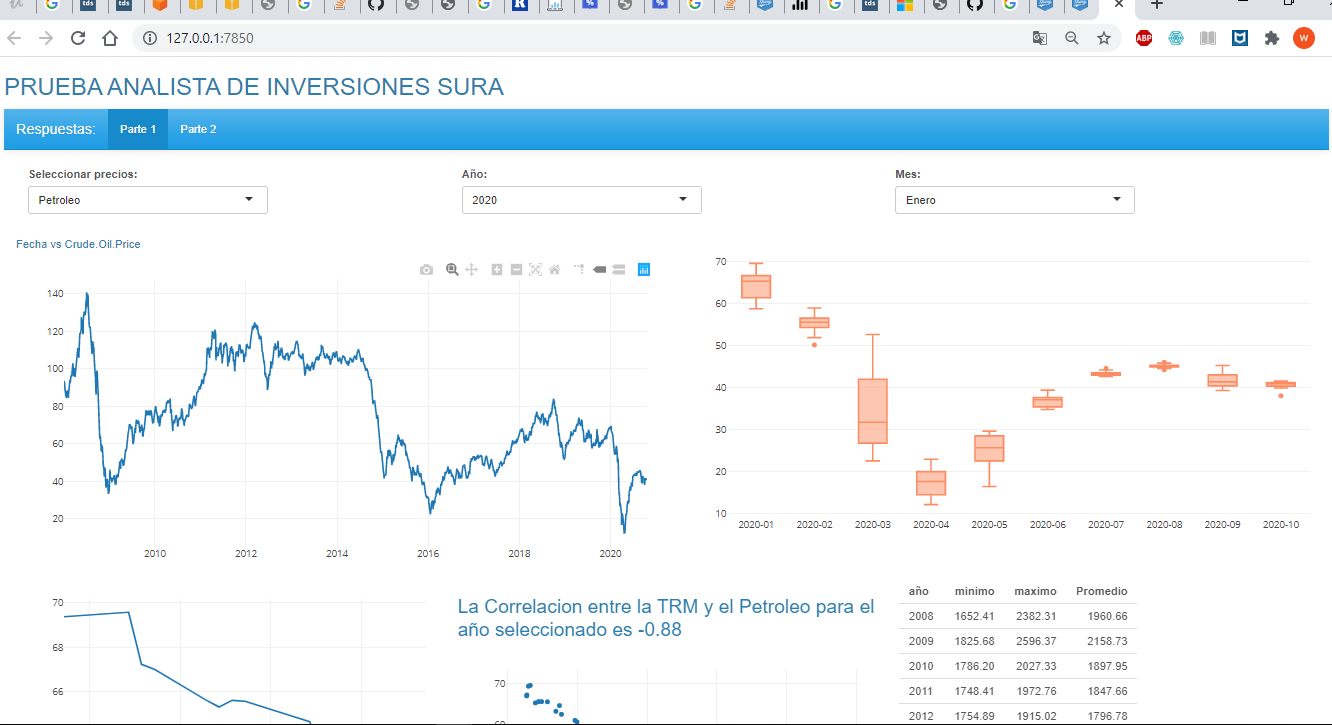
\includegraphics{evidencia/control.png}
\caption{Imagen general}
\end{figure}

De esta forma damos respuesta a las pregunta dadas en los numerales

\begin{figure}
\centering
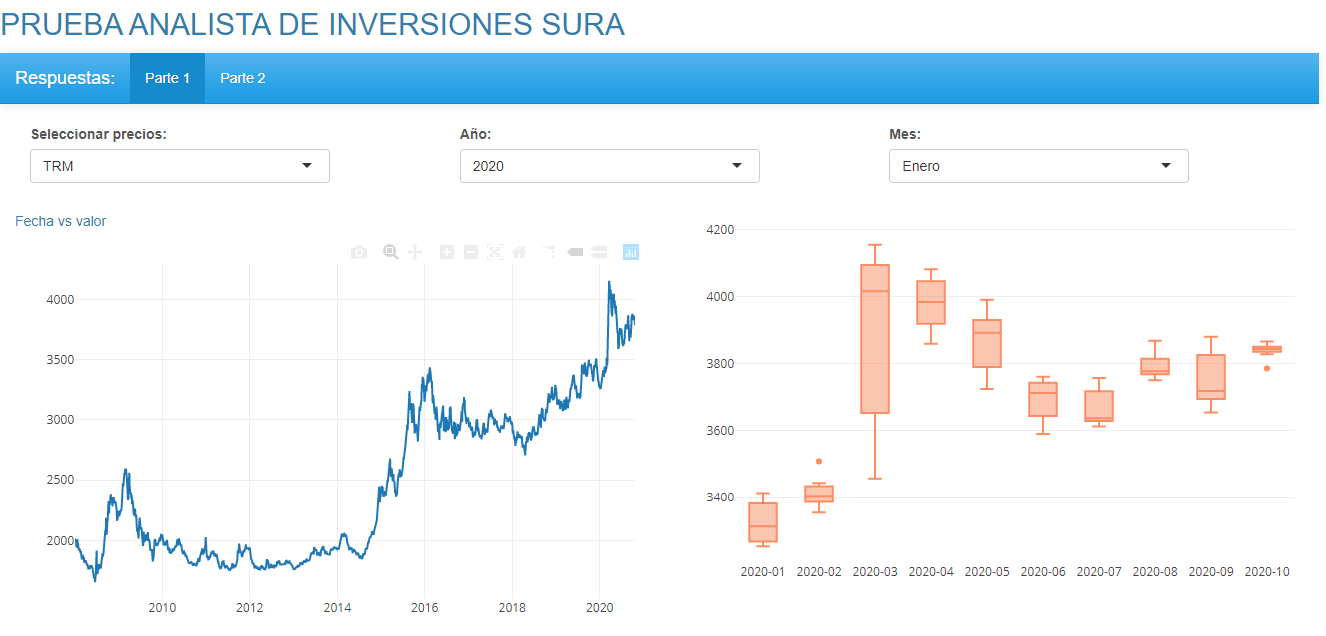
\includegraphics{evidencia/completo1.png}
\caption{Imagen general}
\end{figure}

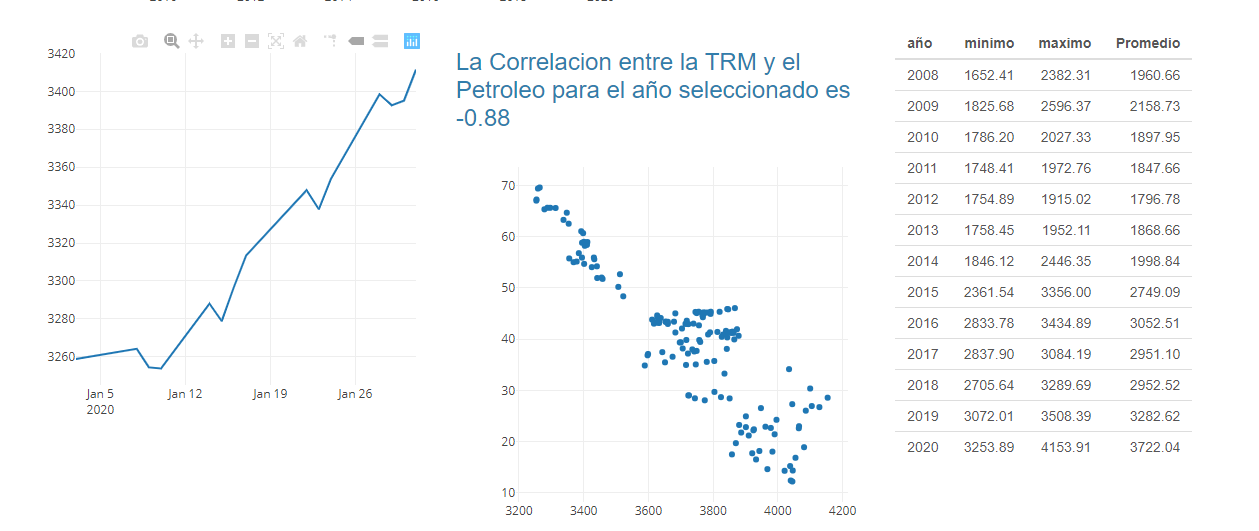
\includegraphics{evidencia/completo2.png} Y mediante el navebar podremos
seleccionar le parte 2 donde seleccionamos algunas de las acciones mas
importantes de S\&P500 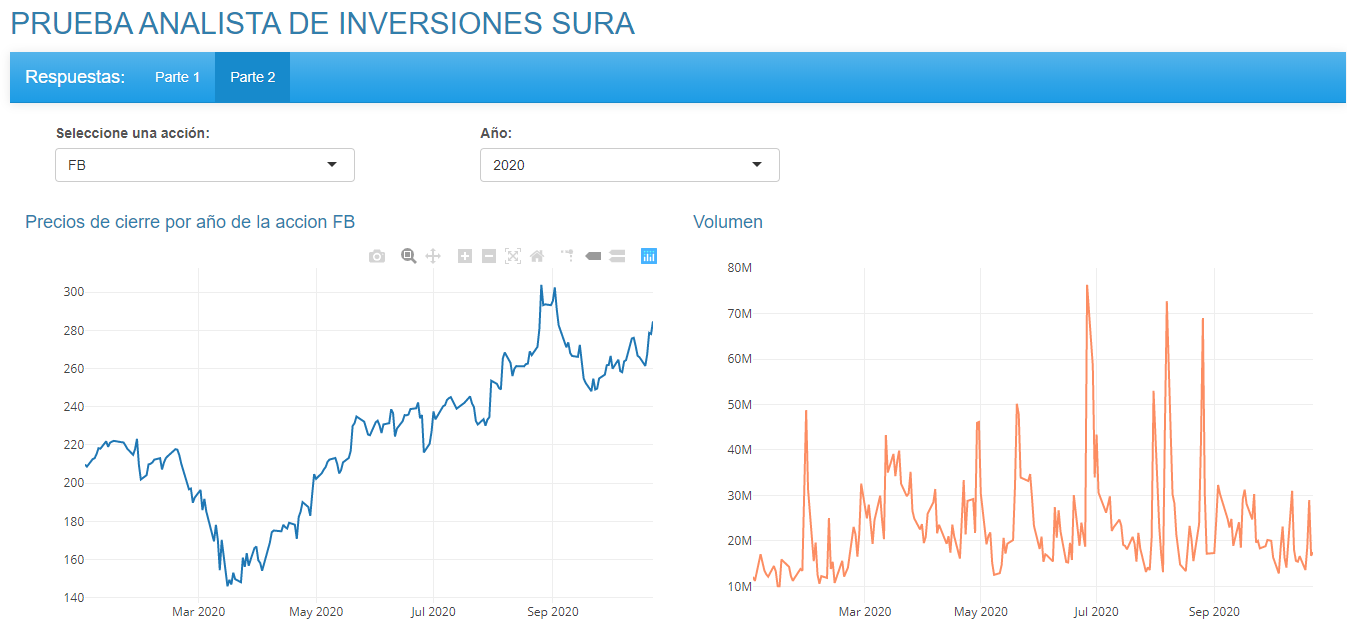
\includegraphics{evidencia/acciones.png} \#\#3.
Las acciones del servidor

En este paso configuramos todos nuestros input reactivos configuramos
nuestras graficas con la libreria seleccionada para hacer las graficas
que fue ploty ejemplo:

bolsa \textless- reactive(\{
financial\_data{[}(financial\_data\(ticker == input\)accion) \&
(financial\_data\(año == input\)yearx),{]}

output\(finanza <- renderPlotly({  plot_ly(bolsa(), y = bolsa()\)price.close
, x = bolsa()\$ref.date , type = `scatter', mode = `lines')

\} )

En este ejemplo de condigo que se repite muchas veces seleccionamos un
dataframe configurados por nuestros input y lo guardamos con la funcion
bolsa() luego renderizamos nuestra grafica en ploty con el dataframe que
se va creando a medica que el usuario marque cada una de las opciones
disponible acciones y año


\end{document}
